
%(BEGIN_QUESTION)
% Copyright 2010, Tony R. Kuphaldt, released under the Creative Commons Attribution License (v 1.0)
% This means you may do almost anything with this work of mine, so long as you give me proper credit

While performing an ``As-Found'' analysis on a control valve equipped with a smart positioner, an instrument technician records this unusual valve signature:

$$\includegraphics[width=15.5cm]{i00746x01.eps}$$

What do you think the unusual ``humps'' in the traces represents?  What physical problem(s) should the technician begin to look for when examining the valve?

\vskip 20pt \vbox{\hrule \hbox{\strut \vrule{} {\bf Suggestions for Socratic discussion} \vrule} \hrule}

\begin{itemize}
\item{} A useful problem-solving technique to apply to any scenario with a graph is to let the graph ``tell you'' what is happening step-by-step in time as you follow it from one extreme to the other.  Try doing this: starting at the lower-left corner, following the upper (red) trace step by step as though you are re-playing the opening of the valve over time, interpreting the graph in terms of stem position and actuator pressure (applied force).  Describe what the graph ``tells'' you as you follow it from one end to the other.
\end{itemize}

\underbar{file i00746}
%(END_QUESTION)




%(BEGIN_ANSWER)

The ``hump'' indicates a sudden change in frictional force from about 58\% to 68\% valve stem travel, but normal friction throughout the rest of the travel.

%(END_ANSWER)





%(BEGIN_NOTES)

The technician should begin looking for anything unusual on the valve stem or valve trim (if cage-guided) causing friction in that range of travel.  Perhaps the stem has been corroded in one spot (rubbing more against the packing between 58\% and 68\% travel) or the piston is grinding against the cage in one spot.

%INDEX% Final Control Elements, valve: diagnostic signature for pneumatic actuator

%(END_NOTES)


